  %% da_manual_EN.tex
  %% Copyright 2015 Simon M. Laube
  %
  % This work may be distributed and/or modified under the
  % conditions of the LaTeX Project Public License, either version 1.3
  % of this license or (at your option) any later version.
  % The latest version of this license is in
  %   http://www.latex-project.org/lppl.txt
  % and version 1.3 or later is part of all distributions of LaTeX
  % version 2005/12/01 or later.
  %
  % This work has the LPPL maintenance status `author maintained'.
  % 
  % The Current Maintainer of this work is S. M. Laube
  %
  % This work consists of the files listed in ./Help/files.txt
  
%%~~~~~~~~~~~~~~~~~~~~~~~~~~~~~~~~~~~~~~~~~~~%% 
%%    Documentation of the etdipa-template   %%
%%~~~~~~~~~~~~~~~~~~~~~~~~~~~~~~~~~~~~~~~~~~~%%
\PassOptionsToPackage{xcolor}{dvipsnames}
\documentclass[12pt,paper=a4]{scrartcl}
\usepackage[utf8]{inputenc}
\usepackage[naustrian,english]{babel}
\usepackage[scale=0.7]{geometry}
\usepackage{graphicx}
\usepackage{float}
\usepackage{circuitikz}
\usepackage{listings}
\usepackage{array}




\lstset{language=[LaTeX]TeX,
		texcsstyle=*\ttfamily\color{red!80!black},
		literate={{ß}{{\ss}}2},
		basicstyle={\ttfamily\color{black}},
		commentstyle=\color{green!60!black},
		keywordstyle=\ttfamily\color{red!80!black},
		numberstyle=\tiny\color{red},
		numbers=left,
		captionpos=b,
		%otherkeywords={},
		basicstyle=\footnotesize,		
		morekeywords={\diplomand ,\breite ,\@width@dpl ,\@sep@dpl,\ifundefined,
					  \@breite,\@default@breite,\setlength,\providecommand,{\ },{\\},\includegraphics,
					  \responsible,\hypersetup,\tikz,\",\href,\node,\dipalistoffigures,$, \{, \}, \[, \],\includepdf,\frontmatter,\appendix,\mainmatter,\schuljahr,\professor,\maketitle,\addchap,\acro,\unterschrift,\usetikzlibrary,\includepdf, \schule,\firma, \Masse,\TikZ,\S,\D,\DS,\SD,\dipacolor,\@@eid@text,\definecolor
\dipalistoffigures,\dipalistoftables,\dplversion,\ETdipaversion,\manversion,\dokumenttyp,\dipvorname,\eidname,\dankname,
\definecolor,\place,\setmyheadings}
		}
		
		\usepackage{etdipa}
		\clearscrheadfoot\relax
		\pagestyle{empty}
		\pagestyle{scrheadings}
		

\setfootsepline{.5pt}
\setheadsepline{.5pt}
\ohead{\today}
\ihead{Simon~Michael~Laube}
\ifoot{{\ttfamily etdipa} -- Manual}
\ofoot{\pagemark}


\title{How to use the {\ttfamily etdipa}-template \ETdipaversion}
\author{Simon~Michael~Laube\\5BHET~2014/15}
\date{\today}
\def\TikZ{Ti\textit{k}Z}
\def\addtoc#1#2{\addcontentsline{toc}{#1}{#2}}
\def\nsec#1{\section*{#1}\addtoc{section}{#1}}
\def\nsubsec#1{\subsection*{#1}\addtoc{subsection}{#1}}
\def\nsubsubsec#1{\subsubsection*{#1}\addtoc{subsubsection}{#1}}
\setlength{\parindent}{0pt}

%% DIRTY TRICK :)
\makeatletter
\def\maketitle{%
\thispagestyle{empty}
\begin{figure}[H]

\includegraphics[scale=1]{Images/ET_logo.jpg}
\centering
\end{figure}
\begin{center}
	\Huge \bfseries\sffamily\@title\\
	\vskip 1em
	\Large\mdseries\rmfamily\@author\\
	\vskip .5em
	\large\mdseries\@date\\
	\normalsize	\rmfamily
\end{center}
				}%
\makeatother

\usepackage[colorlinks=true,
			linkcolor=black,
			citecolor=green,
			urlcolor=blue,
			bookmarks=true,
			bookmarksopen=true]{hyperref}

\begin{document}

\maketitle
\tableofcontents\newpage


\addtocontents{toc}{\protect \large {\bfseries Part~I: Conventions \& Structure}\protect\vspace{1mm}\hrule\normalsize}

\nsec{Introduction}

The {\ttfamily etdipa}-package provides a simple, lightweight
\LaTeX{} template for the documentation of scientific projects.
It is distributed as a whole working directory 
for an arbitrary project\footnote{Please note that the
template is optimized for the {\ttfamily scrreprt} class.}.\par
The motivation for this template was to reach as many
users as possible at different levels of \LaTeX{} knowledge.
Nevertheless some macros are assumed as a minimum requirement
and will be used without any explaination.\par\medskip

The current version is \ETdipaversion{}. It is now possible
to modify several colors and the title page. Further, 
the manual has been translated to English. For additional information
please have a look at the \href{http://www.ctan.org/pkg/etdipa}{README}
file or the complete
\href{https://medium.com/@simon_m_laube/etdipa-offical-release-details-by-the-author-59b6d9ad104b}{project history}.\par \medskip


If there are any suggested improvements, feel free to write an email
using the following adress: \href{mailto:simon.laube@gmx.at}{simon.laube@gmx.at}. Please note that 
this email adress is not intended to be used as a source of information
for the use of this template.\par\medskip
	

\nsubsec{Acknowledgement}
I would like to thank Prof. Mag. Dipl.-Ing. Dr.~Daniel~Asch and Prof. Dipl.-Ing. 
Dr.~Wilhelm~Haager for their help with \TeX nical questions and the supervisory 
of the whole project. Further, I would like to thank everyone who helped improving the template macros and documentation.\par\medskip



\null\hfill -- Simon Michael Laube, \today{} -- 

\section{Conventions}
This section is to briefly summarize the conventions made
for this document.\par\bigskip
\begin{tabular}{>{\bfseries}c l}
Commands &  are written in {\ttfamily typewriter}-font,\\
		&  and within a \textit{listings-} or 
			\textit{verbatim}-environment. \\
&\\
\LaTeX{}-terms&  and emphases are typeset in \textit{italics}.
\end{tabular}\par\bigskip

An overview of all template-specific marcos can be found
in appendix~\ref{sec:befehle}.\par




\section{Structure}

%% ==== Ordner ==== %%
\subsection{Directory structure}
\begin{figure}[H]
\centering
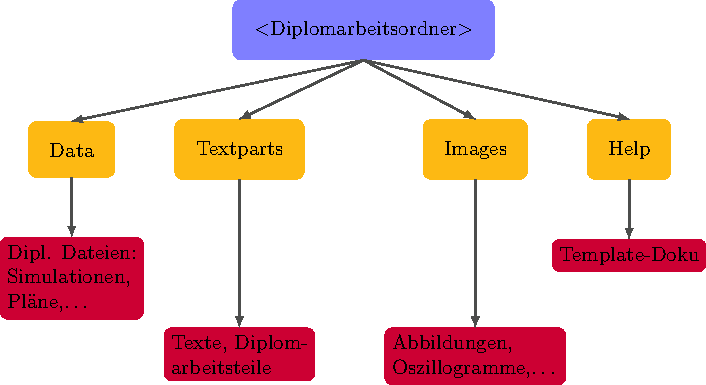
\includegraphics[width=0.7\textwidth]{Images/Ordnerstruktur.pdf}
\caption{Predefined directory structure of the template\newline
		\protect\tikz{\protect\node[rectangle,fill=blue!50!white]{};} \dots\dots master directory\newline
		\protect\tikz{\protect\node[rectangle,fill=yellow!70!red]{};} \dots\dots predefined subfolders\newline
		\protect\tikz{\protect\node[rectangle,fill=red!80!blue]{};} \dots\dots explaination}
\label{pic:ordnerstruktur}
\end{figure}

Figure~\ref{pic:ordnerstruktur} shows the predefined directory structure. The user
should use the master directory \verb|<Diplomarbeitsordner>| as his working 
directory.
All the additional files should be copied to \textit{Data, Images} and \textit{Textparts}.
The \textit{Help} directory contains the template documentation and additional help files.\par\bigskip

When a school or company is using this template, the given structure should not be modified
for reasons of consistency. Nevertheless the users can create subfolders within the given
structure. An example is given in figure~\ref{pic:unterordner}. 
To learn how to work with multiple \LaTeX{} files you should read section~\ref{sec:master}.\par \vspace{1mm}

\begin{figure}[H]
\centering
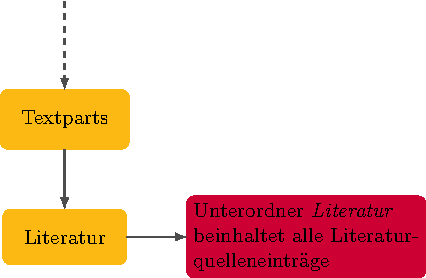
\includegraphics[width=0.4\textwidth]{Images/subordner.pdf}
\caption{An example for creating subfolders within the predefined directories}
\label{pic:unterordner}
\end{figure}

\def\labelitemi{$>$}
\begin{itemize}

\item The \textit{Data} folder contains all the additional data that is not really needed
for the documentation. This could be simulation files (e.g.: Proteus, {\scshape Spice})
as well as technical drawings (e.g.: AutoCAD, \TikZ) or circuit diagrams (e.g.: EPlan).
One could also use this folder to create a separate presentation of the project -- e.g. with 
PowerPoint, Beamer-\LaTeX{}, Prezi or any other program.

\item The \textit{Textparts} folder is the main working directory for your documentation
files. It contains all the sub files of your master document. If you are unsure 
what a master document is, please read section~\ref{sec:master}.

\item The \textit{Images} folder contains all the images of your documentation and work. 
Of course you do not have to include all the files in this folder into your document.

\end{itemize}\bigskip

The master document of your documentation is located in the master directory
of the template. Thus, it is possible to include all the files from your subfolders
into the master document.\par \newpage

%% ==== Mastefile ==== %%
\subsection{Working with master files}\label{sec:master}

Normally a \LaTeX{} document consists of one {\ttfamily *.tex} file. 
Setting up a document that way makes sense,
but if the document gets longer and longer you might loose track of
all the sections and textparts. There is a special technique for
large documents, which is commonly used by real \TeX{}nicians.\par \bigskip


There are two cases:\par 
\begin{itemize}
\item[$-$] The \LaTeX{} file is large, but not too large to loose track of your sections. 
If this is true for you, you can keep your current workflow and create only one \TeX{} file.

\item[$-$] The \LaTeX{} file is very large. In this case you should split your document
into separate files.
\end{itemize}

Since this template is for scientific documents, the second case is true. 
The following \textit{minimal working examples} show how to work with
master and sub files.\par\bigskip

\subsubsection{Standalone documents}
Before someone starts to work with master documents, he/she normally works
with standalone documents, which are basically all the text in one file.
Listing~\ref{lst:normalesarbeiten} shows such a standalone file.\par  


\lstset{caption=A normal \LaTeX{} document,label=lst:normalesarbeiten}
\begin{lstlisting}[ xleftmargin=.14\textwidth, xrightmargin=.14\textwidth]
% documentclass / style
\documentclass{article}
%UTF8 encoding
\usepackage[utf8]{inputenc}
\begin{document}
	\section{Title}
		Here is some text.
		\par % end of the paragraph
\end{document}
\end{lstlisting}


\subsubsection{Master and sub files}
The first step for handling large documents is to create 
a so called \textit{master file}. This file contains
the \LaTeX{} preamble and the start and end of the document.
Listing~\ref{lst:masterfile} shows an example of a
simple master file.\par

\lstset{caption=A simple \LaTeX{} master file,label=lst:masterfile}
\begin{lstlisting}[ xleftmargin=.1\textwidth, xrightmargin=.1\textwidth]
% preamble
\documentclass{article}
\usepackage[utf8]{inputenc}
% document starts here
\begin{document}
	% empty for now
\end{document}
% document ends here
\end{lstlisting}

The second step is to create a \textit{sub file} that only contains
text and sections, but no preamble and no start- or end-of-document command -- see Listing~\ref{lst:subfile}.
Thus, this sub file could not be compiled
by \TeX{}! 

\lstset{caption=A \LaTeX{} sub file,label=lst:subfile}
\begin{lstlisting}[ xleftmargin=.1\textwidth, xrightmargin=.1\textwidth]
%% file: mytext.tex
\section{My text part}
	This is a text part 
	of my large document.\par
\end{lstlisting}\par\vspace{20mm}


To finally create the complete document one has to use the
\TeX{} command \verb|\input|. The argument has to be the relative
path of your sub file based on the absolute path of the master file.\par 
Furthermore a PDF could be included via \verb|\includepdf[<options>]{<name>}|,
but the package {\ttfamily pdfpages} needs to be included for that.
The problem with PDFs is that they have to be scaled
when included, otherwise the header and footer will not fit
the page.
\par

\lstset{caption=\LaTeX{} master file with included subfiles,label=lst:fullmaster}
\begin{lstlisting}[ xleftmargin=.1\textwidth, xrightmargin=.1\textwidth]
% preamble
\documentclass{article}
\usepackage[utf8]{inputenc}
\usepackage{pdfpages}
% document starts here
\begin{document}
	% my first text part %
	\input{mytext.tex}
	% my second text part % as PDF
	\includepdf[pages=3-5]{mypdf.pdf}
\end{document}
% document ends here
\end{lstlisting}

\addtocontents{toc}{\protect\large\protect\newpage{\bfseries Part~II: How to use the template}
\protect \vspace{1mm}\hrule\normalsize}

\section{How to use the macros}\label{sec:macros}
In this section all functions and macros of the 
{\ttfamily etdipa}-template will be explained. The new commands are not
part of the \LaTeX{} standard macros. Therefore, the user
has to use the \verb|etdipa.sty| package to enable the template
macros.\par 


\subsection{Title page -- {\ttfamily maketitle}}

In \LaTeX{} the \verb|\maketitle| command is used
to automatically create the title page from the given
information. The command was redefined for this template to
get a different title page look.
Thus, one can simply say \verb|\maketitle| at the beginning of 
the document and he/she will get the template title page.\par \smallskip

Listing~\ref{lst:maketitle_info} shows the necessary information
that the template-user has to provide.\par 

\lstset{caption=Setup for the title page,label=lst:maketitle_info}
\begin{lstlisting}[xleftmargin=.14\textwidth, xrightmargin=.14\textwidth]
%%==== Setup for the title page ===============%%
\dokumenttyp{DIPLOMARBEIT}
\title{<Title of your work>}
\author{Student 1 \and Student 2}
\place{<Place>}
\date{<Date>}
\schuljahr{<Year>}
\professor{Professor 1 \and Professor 2}
\dipacolor{<Color>}
%%============================================%%
\end{lstlisting}

At the beginning of your document you should 
use \verb|\maketitle| to create the title page.
Next to that the writer should set his
name into the footer via the \verb|\responsible| command.\par 

\lstset{caption=Possible beginning of your document,label=lst:maketitle}
\begin{lstlisting}[xleftmargin=.15\textwidth, xrightmargin=.15\textwidth]
\begin{document}
\frontmatter
%%============ Title page =============%%
\maketitle
% Author of this section
\responsible{Student 1, Student 2}
%%====================================%%
             .     .     .
             .     .     .
             .     .     .
\end{lstlisting}


\subsection{Affidavit}
The affidavit can be added to your document by 
using a predefined environment called \textit{Eid}\footnote{German word
for affidavit}. 
This environment automatically
adds the affidavit text to your document, the only thing
a user has to add is the signature line --
see listing~\ref{lst:eid}. Further, it arranges the 
text at the vertical middle of the page.\par 
\lstset{caption=How to add the affidavit,label=lst:eid}
\begin{lstlisting}[xleftmargin=.15\textwidth, xrightmargin=.15\textwidth]
%%===== Affidavit =======================%%
\begin{Eid}
% adding the signature lines
\unterschrift{Student 1}
\unterschrift{Student 2}
\end{Eid}\newpage
%%=======================================%%
\end{lstlisting}


\subsection{Acknowledgement}

The text of your acknowledgement should be written in an
external file. Again, there is a special environment
for the acknowledgement called \textit{Danksagung}\footnote{German word 
for acknowledgement}.\par 
\lstset{caption=How to add the acknowledgement,label=lst:dank}
\begin{lstlisting}[xleftmargin=.15\textwidth, xrightmargin=.15\textwidth]
%% Acknowledgement
\begin{Danksagung}

% We would like to thank \dots

\end{Danksagung}
\end{lstlisting}

\subsection{References}
References are one of the most important things 
in technical documentations. They should be written in 
a consistent style. \LaTeX{} offers the possibility
to automatically create the reference list out of an
external bibliography file, but this template does
not use this option to keep things a little bit simpler.\par\medskip

The template uses the \LaTeX{} bibliography environment 
with a little modification, so the user has to do less work.
Listing~\ref{lst:literatur} shows how to use the modified
bibliography environment.\par \newpage


\lstset{caption=References,label=lst:literatur}
\begin{lstlisting}[xleftmargin=.15\textwidth, xrightmargin=.15\textwidth]
%% References
\begin{Literatur}

\bibitem[1] % optional number
        {TeXbook}% cite-key
        % text:
        {\textbf{Donald~E.~Knuth:} 
        \emph{The \TeX{}book}. 
        1986, {\scshape Addison--Wesley},
        ISBN-13: 978-0-201-13447-6}
        
\end{Literatur}
\end{lstlisting}
The bibliography entry in listing~\ref{lst:literatur} results in
entry number~\cite{TeXbook}. To refer to a reference one has
to use the \verb|\cite| command.\par 

\lstset{caption=How to cite a bibliography entry,label=lst:zitate}
\begin{lstlisting}[xleftmargin=.15\textwidth, xrightmargin=.15\textwidth]
Text~\cite{<cite-key>}
% for example
Text~\cite{TeXbook}
\end{lstlisting}

\subsection{Acronyms}
The \textit{acronym} package of Tobias~Oetiker~\cite{acronym}
was used to implement the list of acronyms.
Since acronyms are not always necessary, the acronym environment 
was not modified for the template.\par 

\lstset{caption=List of acronyms,label=lst:abkuerz}
\begin{lstlisting}[xleftmargin=.1\textwidth, xrightmargin=.1\textwidth]
% List of acronyms
% Add chapter to contents
\addchap{Acronyms}
\begin{acronym}[ACRONYM] 
% an entry:
%{spi}[SPI]{Serial Peripheral Interface}
\acro{ugs}[ugs.]{umgangssprachlich}                                                                                                                                                                                                                                                                                                                                                                                                                                                                                                                                                                                                                                                                                                                                                                                                                                                                                                                                                                                                                                                                                                                                                                                                                                                                                                                                                                                                                                                                                                                                                               
\end{acronym}\newpage
\end{lstlisting}

The acronym can be used in the text
by calling \verb|\ac{spi}|. At the first
use the whole expansion is shown in the text, 
for all other cases the macro expands to the acronym.\par 


\subsection{Short CV -- the {\ttfamily diplomand} macro}\label{subsec:diplomand}
\begin{figure}[H]
\centering
\diplomand{Max~Mustermann}
		  {12.12.2012 in St.P\"olten}
		  {XY-Street 14}
		  {3100 St.Pölten}
		  {\schule{2010--2015}{HTBLuVA St.Pölten, department for electrical\\ engineering}
		  \schule{2006--2010}{Lower secondary school XY}}
		  {max.muster@xy.at}
		  {Images/bild}
\caption{Result of the short CV command}
\label{pic:diplomandenvorstellung}
\end{figure}\newpage

The short CV can be used to include a short employment and
education history of yourself and every member of the project
into the documentation. The design of the CV is based on the
\LaTeX{} documentclass {\ttfamily moderncv}\footnote{This
documentclass can be used to create high quality 
CVs in different colors and designs.} and was realized via \TikZ{}.\par 


\lstset{caption=How to create a short CV,label=lst:diplomandeneintrag}
\begin{lstlisting}[ xleftmargin=.15\textwidth, xrightmargin=.15\textwidth]
\begin{Diplomandenvorstellung}
   % new CV entry
   \diplomand
   {<Name>}
   {<Date of birth>}
   {<Street and number>}
   {<City and Postal Code>}
   {<Education and employment>} 
   {<Email>}
   {<Path of the picture>}
\end{Diplomandenvorstellung}
\end{lstlisting}

Listing~\ref{lst:diplomandeneintrag} shows how to use the {\verb|\diplomand|}
command. This macro uses the given data and sets up the short CV of
one person. If there are more people working on the project everyone
has to create a short CV. The individual CVs should
be separated with \verb|\newpage|, because every CV arranges itself at
the vertical middle of the page. The command also automatically sets
the person's name into the footer.\par 
\medskip
All 
short CVs must be written within this environment. As mentioned above they 
should be
separated by \verb|\newpage|.
The width of the short CV picture can be changed by 
setting it to another value via \verb|\breite|. 
A default value of $3\,\mathrm{cm}$ is already preset by
the template package.\par 

\lstset{caption=Changing the picture's width,label=lst:breite}
\begin{lstlisting}[ xleftmargin=.2\textwidth, xrightmargin=.2\textwidth]
\breite{<Wert>}
\end{lstlisting}

\subsubsection{Including your previous education or work}
Since version v2.4 there are two new macros that offer
a better possibility to add your employment or education history
to the short CV. Listing~\ref{lst:firma_schule} shows
how the commands can be used.\par 
\lstset{caption=Adding your employment/education history,label=lst:firma_schule}
\begin{lstlisting}[ xleftmargin=.11\textwidth, xrightmargin=.11\textwidth]
\firma{<Period>}{<Name of your job>}
\schule{<Period>}{<Name of your education/school>}
\end{lstlisting}

Although these commands are easy to use, the chronological order 
of the entries must be set 
by the user. Listing~\ref{lst:diplomandenvorstellung} shows
the source code that was used to create 
figure~\ref{pic:diplomandenvorstellung}.\par 

\lstset{caption=An example for a short CV,label=lst:diplomandenvorstellung}
\begin{lstlisting}[ xleftmargin=.15\textwidth, xrightmargin=.15\textwidth]
\begin{Diplomandenvorstellung}
\diplomand{Max~Mustermann}
{12.12.2012 in St.P\"olten}
{XY-Street 14}
{3100 St.P\"olten}
{\schule{2010--2015}{HTBLuVA St.P\"olten, 
department for electrical\\ engineering}
 \schule{2006--2010}{Lower secondary school XY}}
{max.muster@xy.at}
{Images/bild}
\end{Diplomandenvorstellung}
\end{lstlisting}

\subsection{Header and footer}
For the setup of the header and footer the \textit{KOMA-script} package
\verb|scrpage2.sty| is used. The style is defined in the template
package \verb|etdipa| and should not be modified. Do not use
other header-packages than \verb|scrpage2| with \verb|etdipa|,
otherwise you will get warnings or errors.\par 
If the header does not show up in your document you may not have
used the \verb|\mainmatter| or \verb|\frontmatter| command. In this
case you can get the predefined style by using \verb|\setmyheadings| at the
beginning of your document.\par\medskip

The author of a page in the project documentation should always
be listed in the footer. Therefore the \verb|\responsible| 
macro was defined -- see listing~\ref{lst:responsible}.\par 

\lstset{caption=Authors names in the footer,label=lst:responsible}
\begin{lstlisting}[ xleftmargin=.2\textwidth, xrightmargin=.2\textwidth]
\responsible{<Name1>, <Name2>}
\end{lstlisting}\vspace{5mm}



\subsection{Page and chapter numeration}
Mostly documentations consist of three parts. Every part
has a specific page and chapter enumeration. To toggle these
numeration styles some basic \LaTeX{} commands must be used.
\par\newpage

\begin{enumerate}
\item \textit{Frontmatter}, contains everything that is not part of your main text (e.g.: Contents, CV,\dots)
\item \textit{Mainmatter}, contains your main text
\item \textit{Appendix}, contains additional documents like datasheets and so on
\end{enumerate}\bigskip

All the necessary lists -- except for the table of contents -- are located after
the appendix and therefore must be included after the appendix in your master document.\par\medskip


The commands for toggling the enumeration are:
\lstset{caption=Toggling the enumeration within your document,label=lst:nummerierung}
\begin{lstlisting}[xleftmargin=.15\textwidth, xrightmargin=.15\textwidth]
\frontmatter % 
\mainmatter % 
\appendix % 
\end{lstlisting}\par



\newpage
\section{Basic typographical rules}

Every kind of document follows some simple typographical rules. Like Till~Tantau says:
``keep it as simple as possible''~\cite[translated, page\,48--52]{TikZ}). The readers' attention should
be drawn to your text, not to a confusing layout. Thus, you should know some simple rules~\cite{LaTeX}:\par 

\begin{enumerate}

\item Hyphenations are typeset with - \hfill (\verb|-| in \LaTeX{} )\\
	  Domains, e.g. page numbers with ``page\,40--50'' \hfill(\verb|--| in \LaTeX{} )\\
	  Dashes with -- and a space before and after\footnote{That is how it 
	  is done in Europe and the UK, the USA~\cite{TeXbook, LaTeX} is 
	  using---without a space before and after the dash.}
	  \hfill (\verb|--| in \LaTeX{} )\\
	  
\item There should be a small space between a number and its unit. Units are
never typeset in \textit{italics}.\\
 	 e.g.: $I= 12\,\mathrm{A}$\quad\quad (\verb|$I = 12\,\mathrm{A}$|)
 	 
\item Only use acronyms when they are necessary and keep it simple for the reader.

\item Align and numerate long equations (in \LaTeX{} this can be obtained by the math environments \textit{displaymath, align, gather,\dots})
 
\item Use protected spaces that a name is never torn apart into its pieces e.g. \verb|S.~Laube|

\item Use small spaces to make large numbers more readable\\
e.g.: $1.782\,135\,567$ \quad\quad(\verb|$1.782\,135\,567$|)
\end{enumerate}\bigskip

\subsection{Labels and referencing}
Cross referencing is one of the great strenghts of \LaTeX{}.
Thus, one should never write a sentence like: ``{\verb|Figure 1 shows|\dots}''.
This sentence contains two mistakes. At first, \LaTeX{} uses so called \textit{labels} to
get the cross references right. Second, references are always typeset with a protected
space between text and number.\par

A typographically correct cross reference starts when the target element is included into the
document. At that point the user has to set a unique label for this element. Further,
that unique label contains the number of the included element -- for example the label
returns $1$ if your element is the float ``Figure 1''.

\lstset{caption=Setting labels,label=lst:label}
\begin{lstlisting}[xleftmargin=.2\textwidth, xrightmargin=.2\textwidth]
% Sections
\section{Test}\label{sec:test}

% Pictures
\label{pic:test}
% Figures / Diagrams
\label{fig:test}

% Tables
\label{tab:test}
\end{lstlisting}

All the created labels can be used within the text to refer to the desired element --
see listing~\ref{lst:referenz}.\par \medskip

\lstset{caption=Correct cross referencing,label=lst:referenz}
\begin{lstlisting}[xleftmargin=.2\textwidth, xrightmargin=.2\textwidth]

Figure~\ref{pic:test} shows ... 
\end{lstlisting}


\newpage
\appendix
\section{Packages}
The following listing~\ref{lst:packages} shows all the packages
that are by default loaded by the template. Thus, these packages
need not be loaded by the user.\par 

\lstset{caption=Packages loaded by the template,label=lst:packages}
\begin{lstlisting}[xleftmargin=.15\textwidth, xrightmargin=.15\textwidth]
% style
\usepackage[scale=0.75]{geometry}
\usepackage[automark]{scrpage2}
% encoding and fonts
\usepackage[utf8]{inputenc}
\usepackage[T1]{fontenc}
\usepackage{textcomp}
% language
\usepackage[english, naustrian]{babel}
% color
\usepackage[dvipsnames]{xcolor}
% floats
\usepackage{graphicx}
\usepackage{tabularx}
\usepackage{listings,scrhack}
\usepackage[printonlyused,withpage]{acronym}
\usepackage{array}
\usepackage{float}
%TikZ									
\usepackage[europeanresistors,							
            europeaninductors]{circuitikz}
\usetikzlibrary{arrows,automata,positioning}
\usepackage{pgfgantt}
% math packages
\usepackage{amsmath,amssymb}
% others
\usepackage{pdfpages}									 			
\usepackage{etdipa}
\usepackage{todonotes}
% hyperlinks
\usepackage[colorlinks=true,
            linkcolor=black,
            citecolor=green,
            bookmarks=true,
            urlcolor=blue,
            bookmarksopen=true]{hyperref}
\end{lstlisting}\newpage

\section{Template-specific macros}\label{sec:befehle}
\lstset{caption=List of all template-specific macros,label=lst:commands}
\begin{lstlisting}[xleftmargin=.08\textwidth, xrightmargin=.08\textwidth]
% version number
\ETdipaversion 
% puts the author in 
% the footer
\responsible{#1}
% header and footer
\setmyheadings
% title page 
\dokumenttyp{#1}
\and
\professor{#1}
\schuljahr{#1}
\place{#1}
% affidavit
\unterschrift{#1}
% short CV
\firma{#1}{#2}
\schule{#1}{#2}
\diplomand{#1}{#2}{#3}{#4}{#5}{#6}{#7}
\breite{#1}
% colors 
\dipacolor{#1}
ETred
IForange
ELyellow
MBblue
WIgreen
% name variables
\dipvorname
\dankname
\eidname
% affidavit text
\@@eid@text
% environments
\begin{Diplomandenvorstellung}
\end{Diplomandenvorstellung}
\begin{Eid}
\end{Eid}
\begin{Danksagung}
\end{Danksagung}
\begin{Literatur}
\end{Literatur}
%'zero' environments by Prof. Haager
\begin{zeroitemize} % auch mit description und enumerate
\end{zeroitemize}
% lists
\dipalistoffigures
\dipalistoftables
% additional commands
\TikZ 
\Masse % GND Symbol (TikZ)
\S % Y-connection symbol
\D % delta connection symbol
\DS % delta-Y connection symb.
\SD % Y-delta connection symb.
% TabularX-extension by Prof. Haager
L / C / R % as column-type
\end{lstlisting}

\section{Additional information for teachers}
This section is for teachers or supervisors of projects
who use this template. Please read this section before
you introduce the template to your students/colleagues.\par\medskip

The preparation of every part of the documentation
is very essential and should be done carefully. 
\par 

\subsection{Design setup}
At first you should think about the look of the
design you want to use. It is also possible to 
change the look every year or two.\par \medskip

You can either save your setup as a \TeX{} file 
which is then included on top of the documentation -- see section~\ref{sec:master},
or you help your students/colleagues setting up the document rules.\par 

	\subsubsection{Document type}
	On top of your document -- or better: in the preamble -- you need 
	to specify the type of your documentation, for example ``project documentation''
	or ``final exam project'' or something other that fits your project.\par \medskip
	 
	 The standard document type is set to the German word \textit{DIPLOMARBEIT}, but it
	 can easily be changed -- listing~\ref{lst:doctype} shows how.\par 
	 
	 \lstset{caption=Changing the document type,label=lst:doctype}
\begin{lstlisting}[xleftmargin=.1\textwidth, xrightmargin=.1\textwidth]
%% Set document type
\dokumenttyp{DIPLOMARBEIT}% or 
\dokumenttyp{PROJECT DOCUMENTATION}% or
\dokumenttyp{BIOLOGY PROJECT}% anything is possible
\end{lstlisting}
	\subsubsection{Title page}
	A very critical part in your document is the title page. Since it is
	only possible to replace the title picture with the current 
	version~\ETdipaversion{} of this template, you
	will have to have a look at the \LaTeX{} \textit{titlepage} environment
	and the \textit{maketitle} command, if you want to completely change
	the title page look.\par\medskip
	
	The whole document is licensed with the \LaTeX{} Project Public License, so
	you are allowed to modify everything -- including the documentation -- to meet your
	own needs. \par \bigskip
	
	
	\subsubsection{Colors}
	The color of the short CV is another thing supervisors have to worry
	about. This template was originally written for the upper secondary
	school HTL St.Pölten in Lower Austria. Thus, the five department colors
	of the school are predefined by the template:
	\begin{itemize}
		\item ETred
		\item ELyellow
		\item MBblue
		\item IForange
		\item WIgreen
	\end{itemize}
	
	If you do not want to use one of the predefined colors, you could easily
	define your own one, like it is shown in listing~\ref{lst:colordef}.\par 
	
	 \lstset{caption=Defining your own color,label=lst:colordef}
\begin{lstlisting}[xleftmargin=.15\textwidth, xrightmargin=.15\textwidth]
% Color definition
\definecolor{ETred}{RGB}{255,0,0}

% Set the color for your CV
\dipacolor{ETred}
\end{lstlisting}
	
	\subsubsection{Name variables}
	Name variables are an essential feature of the template, since the 
	standard names are in German. The English translation for every
	name variable is automatically set, if the babel option 'english' is used.
	Furthermore the name variables can be changed manually -- see listing~\ref{lst:names}.\par 
	
	 \lstset{caption=Changing name variables,label=lst:names}
	\begin{lstlisting}[xleftmargin=.15\textwidth, xrightmargin=.15\textwidth]
	% Short CV
	\dipvorname{Short student introduction}
	% Acknowledgement
	\dankname{Acknowledgement}
	% Affidavit
	\eidname{Affidavit}
	\end{lstlisting}
	
	
	\subsubsection{Printing}
	In Austria most of the final year project documentations are 
	printed in a one-side format. Nevertheless the twoside option
	is supported by the template and can be used if necessary.
	In case you do not know how two change this option, please
	have a look at listing~\ref{lst:druck}.\par 
	
	 \lstset{caption=The twoside option,label=lst:druck}
	\begin{lstlisting}[xleftmargin=.1\textwidth, xrightmargin=.1\textwidth]
	% twoside option enabled
	\documentclass[twoside,paper=a4,12pt]{scrreprt}
	% twoside option disabled
	\documentclass[paper=a4,12pt]{scrreprt}
	\end{lstlisting}
	
	\subsubsection{Fonts}
	The font for sans-serif texts was changed to be \textit{Helvetica}. All the
	other ones are still the \LaTeX{} default fonts.\par 

 \subsubsection{Affidavit}
 To keep things simple for the user the text for 
 the affidavit is predefined in the \verb|etdipa| package.
 If one would like to change the text\footnote{since this is an English manual you will have to, 
 because the original text is written in German} he or she has to copy
 the \LaTeX{} source code from listing~\ref{lst:eidaendern} into 
 the target document's preamble and add the new text for the affidavit.
 \par \medskip 


\lstset{caption=Changing the text of the affidavit,label=lst:eidaendern}
\begin{lstlisting}[xleftmargin=.15\textwidth, xrightmargin=.15\textwidth]
\makeatletter
     \long\def\@@eid@text{
	               %% put your text here
	            }
\makeatother
\end{lstlisting}

\subsubsection{Leave a note}
There is one thing I want you to do: If your school or company is using
my template officially, please let me know. Just write an email
with the name and city of your institution. I am not going to
publish the information I get from your institution -- the purpose of this
question is to get a personal list of schools/companies that use the template.
Thank you in advance.\par 

\subsection{\TeX nical additions}

\subsubsection{Definition of various dimensions}
The following paragraphs explain the internal dimensions
that were used to create the short CV macro \verb|\diplomand|. An
optical representation of the dimensions can be seen in figure~\ref{pic:bemassungdipl}.\par 

\paragraph{Width of the whole CV.}
The value of this dimension is set to be about
two thirds of \verb|\textwidth|, namely \verb|0.6\textwidth|.
This value should be appropriate for page margins up to $30\%$ --
therefore the scaling factor of the page could be lowered to  $scale=0.7$.
\lstset{caption=Width of the whole short CV,label=lst:ges_breite}
\begin{lstlisting}[ xleftmargin=.15\textwidth, xrightmargin=.15\textwidth]
\newlength{\@width@dpl}
\setlength{\@width@dpl}{0.6\textwidth}
\end{lstlisting}

\paragraph{Distance between picture and frame.}
Another new dimension is the distance between the 
picture and the surrounding frame. The default distance is
$1\,\mathrm{mm}$ and the default line width is \TikZ{}'s internal
default value.
\lstset{caption=Dimension of the frame-picture distance,label=lst:rahmenabstand}
\begin{lstlisting}[ xleftmargin=.15\textwidth, xrightmargin=.15\textwidth]
%Distance picture<->frame
\newlength{\@sep@dpl}
\setlength{\@sep@dpl}{1mm}
\end{lstlisting}

\paragraph{Default width of the picture.} 
To enable any user of this template to change the picture's width the 
\verb|\breite|\footnote{German word for \textit{width}}
macro was defined. Listing~\ref{lst:breite_abfrage} shows how the 
commands and dimensions related to the picture's width were defined 
and how the width could be set by a user.\par\newpage
\lstset{caption=Definition of the picture's width,label=lst:breite_abfrage}
\begin{lstlisting}[ xleftmargin=.14\textwidth, xrightmargin=.14\textwidth]
% macro definition make the 
% width dimension accessible
\let\@breite\relax
\providecommand{\breite}[1]{\gdef\@breite{#1}}

% defining a default value for the width
\newlength{\@default@breite}
\setlength{\@default@breite}{3cm}
% set the value 
\breite{\@default@breite}
\end{lstlisting}

\subsubsection{Dimensions of the short CV}\label{sec:bemassungdipl}
\vspace{-10mm}
\begin{figure}[H]
\centering
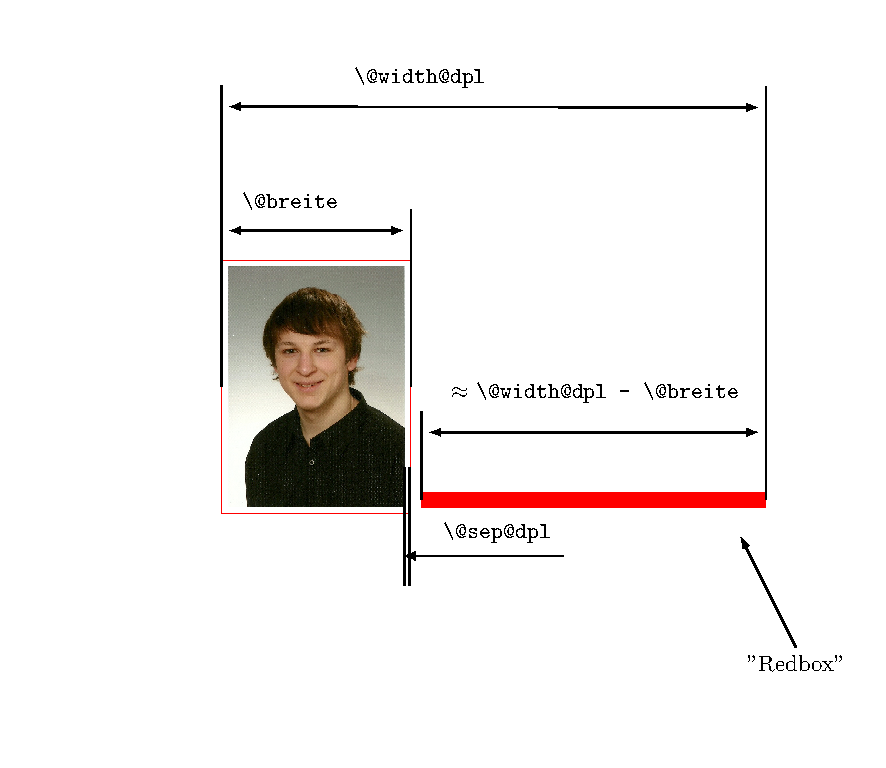
\includegraphics[width=0.8\textwidth]{Images/diplomand_erklaerung.pdf}
\caption{Dimensions within the short CV}
\label{pic:bemassungdipl}
\end{figure}


\textit{Note:} Figure~\ref{pic:bemassungdipl} is to demonstrate
the relations between the different dimensions. As you may notice, there
is a $\approx$ sign in there. That is because even the figure does not 
describe the dimensions as they really are, but it is more likely to
understand the things this way.\par 





\newpage
\def\refname{References}
\phantomsection
\addcontentsline{toc}{section}{\refname}

\begin{thebibliography}{abcd}
\bibitem[1]{TeXbook}{\textbf{Donald~E.~Knuth:} \emph{The \TeX{}book}. 1986, {\scshape Addison--Wesley},\\
ISBN-13: 978-0-201-13447-6} 

\bibitem[2]{LaTeX}{\textbf{Klaus~Braune, Joachim~{\&}~Marion~Lammarsch:}\\
 \emph{\LaTeX{}--Basissystem, Layout, Formelsatz.}
2006, Springer Verlag,\\ ISBN-13: 978-3-540-00718-0}

\bibitem[3]{TikZ}{\textbf{Till~Tantau:} \TikZ{} \emph{and {\scshape pgf}--Manual for version~1.18.} 2007,\\
{\scshape gnu} Free Documentation License, Version 1.2}

\bibitem[4]{clsguide}{\textbf{The \LaTeX 3 Project:} \emph{\LaTeXe{} for class and package writers.}\\
February 2006}

\bibitem[5]{fonts}{\textbf{Carl~G.~Heise:} \emph{\LaTeX{} Kurs: Schriftarten (Kurzeinführung).}\\ TU~Munich, October~2011}

\bibitem[6]{tugboat}{\textbf{Peter~Flynn:} \emph{Rolling your own Document Class:
Using \LaTeX{} to keep away from the Dark Side.} TUGboat, Volume 28 (2007), No. 1}

\bibitem[7]{maketitle}{\textbf{Markus~Kohm:} \emph{Titelseite mit KOMA-Script.} 8.June~2011,\\
found at \url{www.golatex.de/wiki/Titelseite_mit_KOMA-Script}}

\bibitem[8]{headings}{\textbf{Tanja~Richter:} \emph{Fußnoten, Kopf- und Fußzeilen in \LaTeX{}.} May~2004}

\bibitem[9]{acronym}{\textbf{Tobias~Oetiker:} \emph{An Acronym Environment for \LaTeXe .} October~2010}

\bibitem[10]{websites}{\textbf{Public forums:} \url{www.latex-community.org}, \url{www.mrunix.de},\\
									  \url{www.golatex.de}, \url{www.tex.stackexchange.com}, \url{www.texample.net}}
\end{thebibliography}\bigskip

The references above contain all the sources I used to create and document 
the {\ttfamily etdipa}-template. Furthermore they could be useful for any
user of this template.\par 

\end{document}